\section{Preliminaries, Definitions and Known Results}
\label{section_preliminaries} 

We consider the problem of search trees on trees (STTs) which we now describe briefly. For a broader context and additional references, see the works of \cite{BerendsohnThesis, SplayTreesonTrees_andPTAS, TangoSTT, GolinskyThesis}.

The problem of STTs is as follows. We are given a tree topology, and have to construct a search tree (STT) for it where we can search for nodes in response to requests. To answer a request, we make queries on the STT as follows. We start at the root, and query an oracle that tells us whether we found the searched node, or to which direction in the tree (a connected component), with respect to the query, we should proceed. Loosely speaking, the underlying tree and its search tree may have completely different structures, since it is usually beneficial to query a vertex which is not adjacent to $v$ following a query to $v$. But both are trees over the same set of nodes. The cost of a query is the number of oracle queries until the specified node is found.

We focus on the static setting, where the STT is fixed. In this case, we assume that we know the query distribution, $f$ (for frequencies), of the nodes in advance. We want to construct an optimal \emph{static} search tree for $f$. There is also the dynamic setting which we do not consider here, where the STT may be restructured by rotations (appropriately defined). Dynamic algorithms are described in~\cite{BerendsohnThesis, SplayTreesonTrees_andPTAS, TangoSTT}.

We study a specific approach to computing STTs, that is based on linear programming (LP). Our text is self-contained and introduces everything that is necessary for understanding our results. Before we proceed, we give important terminology and definitions, followed by a formal statement of the problem we study.

\begin{definition}[Basic Definitions and Notations]$ $
\label{definitions_basics}
%Basic definitions and notations:

\begin{enumerate}
    \item Node: will always refer to an element of a tree.
    \item Underlying Topology: The topology over which to search. The topology will be consistently denoted as $U$ (for \emph{Underlying}). We  only consider topologies that are trees.
    \begin{enumerate}
        \item We also abuse the notation of $U$ to denote the set of nodes in this tree. Moreover, $n$ will always denote the number of nodes in $U$: $n \equiv |U|$.
        \item For two nodes $i \ne j$, denote by $(i \leftrightsquigarrow j)$ the (unique) path between them in $U$, excluding $i$ and $j$. Use square parenthesis to include $i$ and $j$: $[i \leftrightsquigarrow j]$ (both), $[i \leftrightsquigarrow j)$ (with $i$), $(i \leftrightsquigarrow j]$ (with $j$).
        \item We refer to specific topologies with $2 \le n \le 8$ as $U_{(n,i)}$ where $i$ changes according to the topology. Figure~\ref{figure_all_trees_up_to_n8} (Section~\ref{section_counter_example_main_polytope_study_disproving_conjecture}) and Table~\ref{table_trees_edges} (Appendix~\ref{section_appendix_extras}) show the exact correspondence.
    \end{enumerate}
    
    \item STT: Search tree on tree. We use this term to avoid confusion with the underlying topology which is also a tree. We consistently use $T$ to denote an STT.
    \begin{enumerate}
        \item An STT $T$ is defined over a topology $U$ recursively as follows: Pick a node $r \in U$ and set it to be the root of $T$. Each subtree of $r$  in $T$ is an STT which is  constructed recursively over a connected components of $U \setminus \{ r \}$. See Figure~\ref{figure_topology_to_stt_example} for an example.
        
        \item Frequencies, denoted by $f$: the relative number of queries of each node, a vector of $n$ non-negative values that sum to $1$.
        \item $depth(v)$: The depth of a node $v$ in a given STT is the number of ancestors on its path to the root of the STT, including itself, $depth(root(T))=1$.
        \item $cost(T,f)$: the cost of a (static) STT $T$ with respect to frequencies $f$ is the  sum of the depths of the nodes weighted by their frequencies: $cost(T,f) = \sum_{v \in U} f_v \cdot depth(v)$.
    \end{enumerate}

    \item Linear programming (LP) related:
    \begin{enumerate}
        \item Weights, Direction, Objective (function): may be used interchangeably to describe the objective function of the linear program.
        \item Vertex: always refers to a vertex of the polytope of the linear program (not to be confused with tree nodes).
        %\item $LP(U,w)$: The solution of the LP that is constructed for a topology $U$, with objective (weights) $w$. We abuse notation and use it both for the vertex and its value.
        \item We say that a point is integer if all of its coordinates are integer, and that a polytope is integer if all of its vertices are integer.

        \item We reserve $P$ to denote points in space, and use subscripts such as $P_X$ to denote the projection of $P$ to a set of coordinates $X$. We use $\mathbb{P}$ to denote a collection of points or a polytope. When in need, we use additional capitalized letters to denote points, and their corresponding blackboard-bold font to denote a set of points, for example $S$ and $\mathbb{S}$.
    \end{enumerate}

    \item Cost versus Value: we only use \emph{cost} when we discuss the cost of an STT, and use \emph{value} when we consider the value of a feasible point of the LP with respect to an objective function.
\end{enumerate}
\end{definition}

\begin{figure}[t!]
\centering
    \begin{subfigure}{0.35\textwidth}
        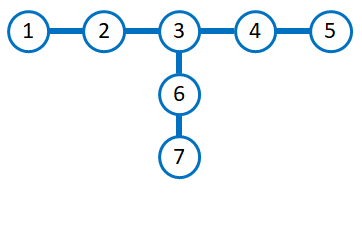
\includegraphics[width=1.0\textwidth]{figure_stt_example-underlying_topology.png}    
    \caption{Underlying tree $U$}
    \label{stt_example_U}
    \end{subfigure}
    ~
    \begin{subfigure}{0.24\textwidth}
        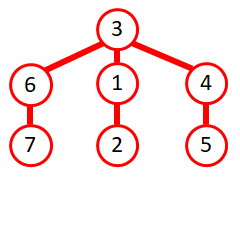
\includegraphics[width=1.0\textwidth]{figure_stt_example-stt1.png}
        \caption{STT $T_1$}
        \label{stt_example_T1}
    \end{subfigure}
    ~
    \begin{subfigure}{0.22\textwidth}
        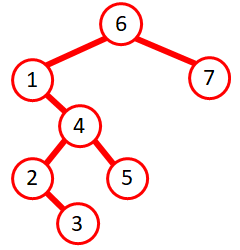
\includegraphics[width=1.0\textwidth]{figure_stt_example-stt2.png}
        \caption{STT $T_2$}
        \label{stt_example_T2}
    \end{subfigure}
    
\caption{\footnotesize{We show two STTs $T_1$ and $T_2$ over the same topology $U$, as described in Definition~\ref{definitions_basics}. 
%There can be many different STTs that correspond to the same topology $U$, among which the simplest STTs are such that we simply root $U$ at some chosen node. In this illustration, the STTs are less trivial.
Note that while while both $U$ and $T_i$ are trees on the same set of nodes, their edges may connect the nodes very differently.
%because an STT may ``jump'' between nodes of the topology.
}}
\label{figure_topology_to_stt_example}
\end{figure}

















\begin{problem}[Static STT]
\label{problem_main_problem_stt}
Let $U$ be a tree topology, and let $f$ be a vector of frequencies. Determine an STT $T$ over $U$ such that $cost(T,f)$ is minimized.
\end{problem}

\subsection{The Linear Program}
\label{subsection_linear_program}


The work of \cite{GolinskyThesis} defines a linear program (LP) formulation to find a $2$-approximation for an optimal solution. The LP uses the following reasoning: Given topology $U$ and the STT $T$ over it, for every pair of nodes, one must be an ancestor of the other, or there is an intermediate node between them that was queried first and acts as their LCA (least common ancestor) in the STT. We define an \emph{ancestry variable} $X_{ij}$ for each pair of nodes  $i,j \in U$ which should take the value $1$ if $i$ is an ancestor of $j$ in $T$, and another variable $Z_{kij}$ which should be $1$ if $k$ is the LCA of $i$ and $j$ in $T$. We only define $Z_{kij}$ for nodes $k \in U$ that are on the path between $i$ and $j$, i.e., $k \in (i \leftrightsquigarrow j)$. Ideally, one would hope to write $Z_{kij} = \min(X_{ki},X_{kj})$ but in an LP formulation we cannot do this, so we are content with writing the inequalities $Z_{kij} \le X_{ki}$ and $Z_{kij} \le X_{kj}$.\footnote{The LP we define soon does not capture additional STT properties, see further discussion in Section~\ref{section_refining_the_LP}.} We can also define the depth variable $D_i = \sum_{(i \ne) j \in U}{X_{ji}}$. The depth represents the cost of search, off by one, such that one aims to minimizes $\sum_{i \in U}{f_i \cdot D_i}$. Ideally we would also require that all of $X$ and $Z$ are either $0$ or $1$, and this would define an integer LP (ILP). However, to be able to rely on LP machinery, we relax this definition and let the variables have non-negative real values.\footnote{Allowing values larger than $1$ is not a problem, because any quantity above $1$ can only hurt the minimization. Bounding each variable only introduces new constraints, so we prefer to ``let the LP do its job'' without it.}
%In addition, we also make another relaxation to be noted later.
To conclude this exposition, the final LP is as follows:

\begin{definition}[STT LP]
\label{definition_LP_program}
A complete description of the LP is as follows:
    \begin{enumerate}
        \item Variables: $X,Z,D$:
            \begin{enumerate}
                \item (Depths) $\forall i \in U: D_{i}$.
                \item (Ancestry) $\forall i,j \in U, i \ne j: X_{ij}$.
                \item (LCAs) $\forall i,j \in U, i \ne j: \forall k \in (i \leftrightsquigarrow j):  Z_{kij}$. Note that $Z_{kij}$ and $Z_{kji}$ are considered as the same variable. (Rather than defining both and equating $Z_{kij}=Z_{kji}$.)
            \end{enumerate}
        \item Constraints:
        \begin{enumerate}
            \item (Bounds\footnote{Technically we can omit the non-negativity constraints on $Z$, since $Z$ is not part of the objective and can only ``help'' the ancestry-constraints when it is non-negative. Alternatively, we can keep $Z \ge 0$ and have the non-negativity of $X$ implied by the loosely-LCA constrains. We cannot omit both sets, since then the LP becomes unbounded.}) $\forall i,j \in U: \forall k \in (i \leftrightsquigarrow j): 0 \le X_{ij},X_{ji},Z_{kij}$.
            \item (Ancestry) $\forall i,j \in U: X_{ij} + X_{ji} + \sum_{k \in (i \leftrightsquigarrow j)}{Z_{kij}} \ge 1$.
            \item (Loosely LCA) $\forall Z_{kij}: (1) \; Z_{kij} \le X_{ki} \ \ \ ; \ \ \ (2) \; Z_{kij} \le X_{kj}$.
            \item (Depth) $\forall i \in U: D_i \ge \sum_{(i \ne) j \in U}{X_{ji}}$.
        \end{enumerate}
        \item Objective function: minimize $f \cdot D = \sum_{i \in U}{f_i \cdot D_i}$.
    \end{enumerate}
\end{definition}

Observe that we relaxed the ancestry and depth constraints to be inequalities, rather than equalities, even though STTs satisfy them with equalities.
%%% [Omitted for space considerations]
%%% On the one hand, equalities reduce the space of solutions, so it may be beneficial to keep them. On the other hand, since we already deal with a minimization problem it does not hurt to have inequalities, and in fact leaving this extra freedom will likely be safer when we later practically solve the LP numerically in some cases.


\begin{remark}
\label{remark_lp_variables_all_viewed_as_LCA}
$X$ and $Z$ seem to serve slightly different roles. A canonized way to look at them is by adding variables of the form $Z_{iij}$ to represent $i$ being the LCA of $i$ and $j$. In this case $X_{ij} = Z_{iij}$, and the ancestry inequality becomes $\forall i,j: \sum_{k \in [i \leftrightsquigarrow j]}{Z_{kij}} \ge 1$. If we wish, we can also define $Z_{iii}$ and have an ancestry inequality for $i=j$, which would imply $Z_{iii} \ge 1$ (every node is its own ancestor) and redefine $D_i \ge \sum_{j \in U}{Z_{jji}}$ so that the STT depth and the LP depth are the same. All of this being said, we stick to the separated presentation of the $X$ and $Z$ variables, particularly because $Z$ is a little more artificial (see Section~\ref{subsection_with_and_without_z_fourier_motzkin}).
\end{remark}



\subsection{Conjectures and Known Results}
In this subsection we summarize important facts regarding the LP, all were proven in \cite{GolinskyThesis}.

\begin{definition}[STT Induced Point]
\label{definition_xzd_of_stt}
Let $T$ be an STT. We denote by $(X^T,Z^T,D^T)$ the LP variables it induces: $X_{ij}=1$ if $i$ is ancestor of $j$, $Z_{kij}=1$ if $k = LCA(i,j)$ in $T$. The rest of the $X,Z$ variables are $0$, and $\forall i \in U: D_i = \sum_{j \in U\setminus \{ i \}}{X_{ji}}$.
\end{definition}

\begin{property}[Trees are Feasible]
\label{property_stt_feasible}
Let $T$ be an STT. Then $(X^T,Z^T,D^T)$ is a feasible solution. Moreover, the ancestry and depth inequalities are tight (equalities).
\end{property}

\begin{remark}[Depth Discrepancy]
\label{remark_depth_off_by_one}
Let $T$ be an STT. Observe that $\forall v \in U: depth(v) = D^T_v + 1$. This means that we can relate the cost of the STT to the value of the LP on the point it induces: $cost(T,f) = \sum_{v \in U}{f_v \cdot depth(v)} = \sum_v{f_v} + f \cdot D$. If $f$ is a vector of weights and not frequencies, first normalize it. Throughout the text, we usually deal with depths of the LP (the $D$ variables), and it is fine since we know how to relate them to the actual STT depths and its cost.
\end{remark}



\begin{property}[Integer Domination]
\label{property_integer_domination}
Let $(X',Z',D')$ be an \emph{integer} feasible solution. Then there exists an STT $T$, which can be computed efficiently, such that $\forall i \in U: D^T_i \le D'_i$. Alternatively phrased: the Integer-LP has an optimum that corresponds to an STT.
\end{property}

\begin{property}[$2$-Approximation]
\label{property_tree_2_approx}
Let $(X',Z',D')$ be \emph{any} feasible solution. Then there exist an STT $T$, which can be computed efficiently, such that $\forall i \in U: D^T_i \le 2 \cdot D'_i$.
\end{property}

Both Property~\ref{property_integer_domination} and Property~\ref{property_tree_2_approx} are proven constructively in \cite{GolinskyThesis}. The STT that achieves these guarantees is computed by the following rounding scheme. Note that this scheme not only rounds all the coordinates to be integer, it also takes integer solutions and ``rounds'' them to STTs.

\begin{definition}[Conversion to STT: Root Rounding]
\label{definition_rounding_scheme}
Let $U$ be a tree topology, and let $P = (X,Z,D)$ be the solution found by the LP for some weights. ${STT}_U(P)$ is the search tree on $U$ that is computed recursively as follows.
If $U$ has a single node, then we have a trivial singleton search tree. Otherwise, find a node $r$ such that: $\forall v (\ne r) \in U: \sum_{u \in U:r \in [u \leftrightsquigarrow v)}X_{uv} \ge \frac{1}{2}$. We clarify that $r \in [u \leftrightsquigarrow v)$ means that $r$ is on the path between $u$ and $v$, and may be $u$ (but not $v$). \cite{GolinskyThesis} proves that such a node exists. Set $r$ as the root of $STT_U(P)$, and construct its subtrees ${STT}_H(P)$  for each connected component $H \subseteq U \setminus \{r\}$ recursively. We refer to this rounding method as \emph{root rounding} or simply \emph{rooting}.
\end{definition}

Intuitively, the choice of the root guarantees that some of the (fractional) depth of each node $v$ is due to nodes that are $r$ or belong to a different connected component than the one of $v$, when $r$ is removed (so we charge $r$ for them). Because of this, setting $r$ to be the root increases the depth of any node $v \ne r$ by at most $\frac{1}{2}$ compared to
its fractional depth $D_v$ which we know by the choice of $r$ is at least $\frac{1}{2}$ for every $v \ne r$. For a formal proof that such $r$ always exists, see Lemma 3.4 in \cite{GolinskyThesis}. We emphasize that there may be multiple choices for the root at any given step, so the resulting STT and its approximation ratio may depend on the tie breaking rule.


Property~\ref{property_integer_domination} (Theorem 3.1 of \cite{GolinskyThesis}) implies that when considering integer solutions, there is an optimal solution that is indeed a search tree (in fact, it is a vertex of the LP). Property~\ref{property_tree_2_approx} (Theorem 3.2 of \cite{GolinskyThesis}) implies that the feasible point corresponding to an optimal STT is a $2$-approximation for the LP optimum. Golinsky \cite{GolinskyThesis} conjectured the following.

\begin{conjecture}[Conjecture 3.1 of \cite{GolinskyThesis}]
\label{conjecture_LP_finds_STT_vertex}
For any topology and any vector of non-negative weights, there is an optimal STT that induces an optimal solution to the LP in Definition~\ref{definition_LP_program}.
\end{conjecture}

Conjecture~\ref{conjecture_LP_finds_STT_vertex} implies that all the vertices of the LP are STTs, since by Theorem~\ref{theorem_integer_vertex_iff_stt} every vertex has some objective for which it is uniquely optimal.
In the language of polytopes and extended formulations~\cite{ExtendedFormulationSurvey}, Conjecture~\ref{conjecture_LP_finds_STT_vertex} states that the LP in Definition~\ref{definition_LP_program} is an extended formulation of an original polytope of interest. The original polytope is the convex hull of all STTs in $n$ dimensional $D$-space (depth per node), and the LP is (conjectured to be) an extended formulation with additional $X$ and $Z$ variables.

Since we care about Problem~\ref{problem_main_problem_stt} and the LP is just a tool, a weaker conjecture is as follows.

\begin{conjecture}
\label{conjecture_LP_rounding_finds_opt_STT}
For any topology and any vector of non-negative weights, rounding an optimal solution of the LP in Definition~\ref{definition_LP_program}, according to the root rounding scheme (Definition~\ref{definition_rounding_scheme}) yields an optimal STT.
\end{conjecture}

The work~\cite{GolinskyThesis} verified the conjectures for trees up to $n \le 4$ nodes, and lists several ideas and failed directions for a general proof. One hope to prove Conjecture~\ref{conjecture_LP_finds_STT_vertex} would be to show that all the vertices of the LP correspond to STTs, but this is not the case as we show in Theorem~\ref{theorem_non_tree_vertex}.

\textbf{We disprove both conjectures.} In simple words, we show that there exist tree topologies and frequencies such that the value of the best STT for them is strictly larger than the LP optimum, and that the rounding scheme might, and sometimes always, yield a sub-optimal STT. In particular, such optimum of the LP must be a non-integer solution by Property~\ref{property_integer_domination}.
